%
% separation.tex
%
% (c) 2019 Prof Dr Andreas Mueller
%
\lhead{Separation of Variables}
\rhead{}
\chapter{Separation of Variables\label{chapter:separation}}
\index{stroboscope}
\index{standing wave}
\begin{figure}
\begin{center}
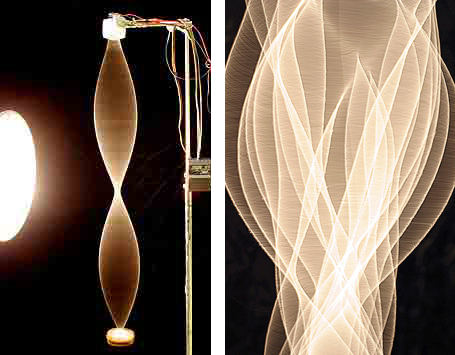
\includegraphics[width=0.8\hsize]{../common/graphics/stringvibrlarge-10-06-06.jpg}
\end{center}
\caption{
Vibrating string
(Image by A.~Davidhazy, http://people.rit.edu/andpph/)
\label{separation:schwingendesaite}}
\end{figure}
Lighting a vibrating string with a stroboscope at the frequency of the
string makes the string seemingly stand still (see figure
\ref{separation:schwingendesaite})
The shape of the solution of the wave equation thus is the same
at periodically recurring points in time.
Measuring the elongation's dependence on time, it turns out to be
a harmonic oscillation which can be described using sine and cosine
functions.
This leads to the conjecture that the solution can be written as 
a product
\[
u(x,t)=X(x)\cdot\sin\omega t\quad\text{oder}\quad X(x)\cdot\cos\omega t.
\]
The goal of this chapter is to develop this idea into a solution
algorithm that is applicable to a suitably large class of partial
differential equations.

%
% ode.tex -- XXX
%
% (c) 2019 Prof Dr Andreas Müller, Hochschule Rapperswil
%
\section{Differentialgleichungen zweiter Ordnung}
Das Standardverfahren für die Lösung einer gewöhnlichen linearen
Differentialgleichung mit konstanten Koeffizienten
\[
a_2y''+ a_1y'+a_0y=0
\]
schreibt vor, dass man erst die Nullstellen $\lambda_{1,2}$
des charakteristischen Polynoms
\[
p(\lambda)=a_2\lambda^2+a_1\lambda+a_0
\]
finden muss.
Die allgemeine Lösung der Differentialgleichung ist dann
eine Linearkombination
\[
y(x)=
A_1 e^{\lambda_1t}
+
A_2 e^{\lambda_2t},
\]
die Konstanten $A_1$ und $A_2$ sind aus den Anfangswerten zu bestimmen.
Sinde $y_0$ und $v_0$ der Anfangswert und die Anfangsableitung, dann
findet man das lineare Gleichungssystem
%\newcolumntype{\linsysR}{>{$}r<{$}}
%\newcolumntype{\linsysL}{>{$}l<{$}}
%\newcolumntype{\linsysC}{>{$}c<{$}}
%\newenvironment{linsys}[1]{%
%\begin{tabular}{*{#1}{\linsysR@{\;}\linsysC}@{\;}\linsysR}}%
%{\end{tabular}}
\[
\begin{linsys}{3}
         A_1&+&         A_2&=&y_0\phantom{.}\\
\lambda_1A_1&+&\lambda_2A_2&=&v_0.
\end{linsys}
\]
Besonders einfach wird die Bestimmung jedoch für die Differentialgleichung
\[
y''+k^2 y=0.
\]
Dann sind die $\lambda_{1,2}=\pm\sqrt{-k^2}$ imaginär, und man kann statt
der Exponentiallösungen auch den Ansatz
\[
y(x)=A\cos kx+B\sin kx
\]
verwenden.
Da der Wert von $\sin kx$ bei $x=0$ verschwindet, und die Ableitung von
$\cos kx$ ebenfalls, ist die Bestimmung der Konstanten viel einfacher:
\[
A=y_0
\qquad\text{und}\qquad
B=\frac1kv_0,
\]
oder
\begin{equation}
y(x)=y_0\cos kx + \frac{v_0}{k}\sin kx
\label{hyp:loesung}
\end{equation}

Für die analoge Differentialgleichung $y''-k^2y=0$ geht dies nicht.
Die Nullstellen des charakteristischen Polynoms sind hier 
$\lambda_{1,2}=\pm k$, und es führt nichts an dem linearen Gleichungssystem
\[
\begin{linsys}{3}
 A_1&+& A_2&=&y_0\\
kA_1&-&kA_2&=&v_0
\end{linsys}
\]
vorbei.
Die Lösung kann allerdings zum Beispiel mit dem Determinantenverfahren
ziemlich direkt gefunden werden:
\begin{align*}
A_1
&=
\frac{\left|\begin{matrix}y_0&1\\v_0&-k\end{matrix}\right|}{\left|\begin{matrix}1&1\\k&-k\end{matrix}\right|}
=
\frac{-ky_0+v_0}{-2k},
&
A_2
&=
\frac{\left|\begin{matrix}1&y_0\\k&v_0\end{matrix}\right|}{\left|\begin{matrix}1&1\\k&-k\end{matrix}\right|}
=\frac{v_0-ky_0}{-2k}.
\end{align*}
Damit kann man jetzt die Lösung auch in diesem Fall hinschreiben:
\begin{align}
y(x)
&=
A_1e^{kx}+A_2e^{-kx}
=
\frac12\biggl(
\frac{ky_0-v_0}k e^{kx}
+
\frac{-v_0+ky_0}k e^{-kx}
\biggr)
\notag
\\
&=
y_0\frac{e^{kx}+e^{-kx}}2
+\frac{v_0}{k}\frac{e^{kx}-e^{-kx}}2.
\label{hyp:hyperbelfunktionen}
\end{align}
Die Erfüllung der Anfangsbedingung könnte also auch in diesem Falle
sehr einfach sein, wenn man nicht die Funktionen $e^{\pm kx}$ verwenden
würde, sondern deren Linearkombinationen wie in (\ref{hyp:hyperbelfunktionen}).


%
% idea.tex -- idea of the method
%
% (c) 2008 Prof Dr Andreas Mueller
%

\section{Idea of the method}
In applications one often has some indications from the application
domain what the solution function will most probably look like, or one
is looking for a very particular type of solution.
In particular, the dependence of the solution on one of the variables may be
known up to a factor depending only on the other variables.
In these situations one can try to write the solution as a product
or sum of functions that depend on only one variable.

Even if one knows nothing about the solution, one can still try such
an {\em ansatz}, as the following example tries to illustrate.
Let's attempt to solve the partial differetnial equation
\begin{equation}
\frac1x
\frac{\partial u}{\partial x}
+
\frac1y
\frac{\partial u}{\partial y}
=\frac1{y^2}
,
\qquad x>1, y>1,
\label{separation:beispiel1}
\end{equation}
ignoring the boundary conditions for the time being.
We try to represent the solution as a sum of two functions which depend
on one of $x$ and $y$ only.
\begin{equation}
u(x,y)=X(x)+Y(y)
\quad\Rightarrow\quad
\begin{cases}
\quad{\displaystyle \frac{\partial u}{\partial x}}&=X'(x)\\
\\
\quad{\displaystyle \frac{\partial u}{\partial y}}&=Y'(y)\\
\end{cases}
\label{separation:beispiel1:ansatz}
\end{equation}
Substituting this into the differential equation
(\ref{separation:beispiel1})
gives the new equation
\[
\frac{X'(x)}{x}+\frac{Y'(y)}{y}=\frac1{y^2}
\]
or
\begin{equation}
\frac{X'(x)}{x}
=\frac1{y^2}
-\frac{Y'(y)}{y}.
\label{separation:beispiel1:separiert}
\end{equation}
The form (\ref{separation:beispiel1:separiert}) has a distinct property:
the variable $x$ only appears on the left side, the variable $y$ only on
the right.
If we fix some value $y$, the right hand side cannot change, so the left
hand side must not depend on $x$.
Conversely, if we fix $x$, then the left side cannot change any more,
and thus the right hand side cannot change either.
We conclude that both sides must be the same constant.
Calling this constant $k$ we find the two ordinary differential equations
\begin{align}
\frac{X'(x)}{x}&=k
&
k&=\frac1{y^2}-\frac{Y'(y)}{y}
\label{separation:beispiel1:separiertedgl}
\end{align}
for $X(x)$ and $Y(y)$.

The differential equation for $X$ is easy to solve:
\begin{align*}
X'(x)&=kx\quad\Rightarrow\quad X(x)=
\frac12kx^2+C_x.
\end{align*}
The right equation is only slightly more complicated:
\begin{align*}
Y'(y)=\frac1y-ky
\quad\Rightarrow\quad
Y(y)=\int\frac1y-ky\,dy=
\log y-\frac12ky^2+C_y.
\end{align*}
We can now combine these functions into a solution of the initial
differential equation:
\begin{equation}
u(x,y)=
\frac12kx^2+
\log y-\frac12ky^2+C.
\label{separation:beispiel1:loesung}
\end{equation}
By varying the parameters $k$ and $C$, formula
(\ref{separation:beispiel1:loesung}) gives an infinite family of
solutions of the partial differential equation.
The values of these constants need to be determined by boundary conditions
in a manner to be studied later.

Let's summarize the method so far:
\begin{enumerate}
\item
Choose an {\em ansatz} from functions that depend from disjoint
sets of variables.
\item
Substitute into the partial differential equation and separate terms
involving the separate sets of variables.
The two sides of the equation depend on disjoint sets of variables
und must therefore be constant.
\item 
Split the equation into two coupled equations, each with a
different set of independent variables.
\item
Solve each equation individually.
\item
Put solutions together using the boundary conditions.
\end{enumerate}
As may suspected, the problem most of the time is not the solution
of the individual equations but rather the last step.
In the following sections we want to illustrate how this can be
done in a variety of examples.


%
% lpde.tex -- why linear pdes?
%
% (c) 2019 Prof Dr Andreas Mueller
%
\section{Separation for linear partial differential equations}
The base idea of the separation method produces a family of functions
that depend an some integration and separation constants.
On the boundary we are usually given some arbitrary functions.
In general it will be impossible to tune these few constants to
values that reproduce the boundary functions.
This basic version of the separation method thus is incapable of
solving a general partial differential equation due to the lack
of flexibility in the set of solutions found.

This problem changes if different solutions can be combined into new ones.
Linear combinations of solutions introduce a large set of additional
parameters to tune the solution.
In particular, Fourier theory shows that linear combinations of
basic functions can be tuned to approximate just about any periodic
function.
However, linear combinations of solutions are in general no longer
solutions the equation, except for linear partial differential
equations.
This is expressed in the following theorem.

\begin{satz}
If $u_1$ and $u_2$
are solutions of a homogeneous linear partial differential equation,
then $u_1+u_2$ and $\lambda u_1$ with $\lambda\in\mathbb R$ are also
solutions.
\end{satz}

\begin{proof}
The differential equation
\[
F(x_1,\dots,x_2,u,\frac{\partial u}{\partial x_1},\dots)=0
\]
is linear in $u$ and its derivatives, so we can expand sums and
pull factors from inside $F$:
\begin{align*}
F(x_1,\dots,x_2,u_1+u_2,\frac{\partial u_1}{\partial x_1}+\frac{\partial u_2}{\partial x_1},\dots)
&=
F(x_1,\dots,x_2,u_1,\frac{\partial u_1}{\partial x_1},\dots)
\\
&+
F(x_1,\dots,x_2,u_2,\frac{\partial u_2}{\partial x_1},\dots)=0
\\
F(x_1,\dots,x_2,\lambda u_1,\frac{\partial \lambda u_1}{\partial x_1},\dots)
&=
\lambda
F(x_1,\dots,x_2,u_1,\frac{\partial u_1}{\partial x_1},\dots)
=0
\end{align*}
Thus linear combinations of $u_1$ and $u_2$ are solutions too.
\end{proof}

Linear cominations allow us to first find as many different solutions
$u_1$, $u_2$, $u_3,\dots$ and then to use suitable coefficients $a_k$
to combine them into a solution
\[
u(x)=\sum_{i=1}^\infty a_ku_k
\]
that also satisfies the boundary conditions.

Inhomogeneous linear partial differential equations can be solved using
this method too.
As pointed out in chapter~\ref{chapter:terminology and notation},
we first have to find a particular solution $u_p$ which solves the
inhomogeneous partial differential equation independently
of any boundary conditions.
The separation method can be helpful for this too.
Then the problem is reduced to finding a solutions $u_h$ to the homogeneous
equations with boundary condition $g-u_p$ on $\partial\Omega$.
Using the separation method, we can build up $u_h$ as a linear combination
of solutions.

The coefficients $a_k$ for the linear combination often lead us into
Fourier theory or some generalization of it.
Such partial solutions often have immediate physical significance.
In mechanical or electrical engineering they appear as vibration modes,
in quantum mechanics as energy states.



%
% membrane.tex -- XXX
%
% (c) 2019 Prof Dr Andreas Mueller
%
\section{Vibrating rectangular membrane}
\rhead{Rectangular Membrane}
Let's consider the vibration of a rectangulare membrane fixed on
the boundary of the domain
\[
R=\{(x,y)\,|\,0\le x\le a,0\le y\le b\} =(0,a)\times(0,b).
\]
At time $t=0$, the shape of the membrane is given by a function
$f(x,y)$ defined on $R$.
For arbitrary times $t\ge 0$ it is described by a function $u(x,y,t)$ 
with differential equation
\[
\frac1{c^2}\frac{\partial^2u}{\partial t^2}=\frac{\partial^2u}{\partial x^2}+\frac{\partial^2u}{\partial y^2}
\]
and satisfies the boundary conditions
\begin{align*}
u(x,y,0)&=f(x,y)\quad\forall 0\le x\le a,0\le y\le b,
\\
\frac{\partial}{\partial t}u(x,y,0)&=g(x,y)\quad\forall 0\le x\le a,0\le y\le b
\end{align*}
at time $t=0$ and
\begin{align*}
u(0,y,t)&=0&u(a,y,t)&=0&\forall t\ge 0,0\le y\le b,\\
u(x,0,t)&=0&u(x,b,t)&=0&\forall t\ge 0,0\le x\le a.
\end{align*}
around the boundary of $R$.

\subsection{Separating Time}
We want to separate variable $t$ from the rest of the variables.
According to the ideas expanded in the introduction to this chapter,
we try to stuff the time dependence into a separate function $T(t)$,
and the dependence on $x$ an $y$ in $\varphi(x,y)$.
We thus use the ansatz
\[
u(x,y,t)=T(t)\cdot\varphi(x,y).
\]
It will obviously not be possible to describe every vibrating membrane
with just one such function.
We thus expect to find a sufficiently large set of partial solutions
that will allow us to tune a linear combination to also satisfy the 
initial conditions.


In any event, the boundary conditions along $\partial R$ do not depend
on time, so we need that the function $\varphi$ satisfies the following
boundary conditions:
\begin{align*}
\varphi(0,y)&=0&\varphi(a,y)&=0&0\le y\le b\\
\varphi(x,0)&=0&\varphi(x,b)&=0&0\le x\le a
\end{align*}

Now let's substitute the ansatz for $u$ into the wave equation.
We obtain:
\[
\frac1{c^2}T''(t)\varphi(x,y)=T(t)\left(
\frac{\partial^2\varphi}{\partial x^2}
+
\frac{\partial^2\varphi}{\partial y^2}
\right).
\]
We are looking for a function $u$ that does not vanish identically,
thus points where $T$ vanishes are isolated.
Also the points where $\varphi(x,y)$ vanishes form a set of area $0$,
so in most points, it is perfectly OK to devide by $T(t)$ and
$\varphi(x,y)$.
This turns the equation into
\begin{equation}
\frac1{c^2}\frac{T''(t)}{T(t)}
= \frac1{\varphi(x,y)}\left( \frac{\partial^2\varphi}{\partial x^2}
+ \frac{\partial^2\varphi}{\partial y^2} \right)
\label{separiertMembran}
\end{equation}
The right hand side depends only on $(x,y)$, the left hand side only on $t$.
According to the basic principle of the separation method, both sides
must be constant.
There is therefore a $k$ with the property
\[
\frac1{c^2}\frac{T''(t)}{T(t)}=k
\qquad\Leftrightarrow\qquad
T''(t)=k T(t).
\]
This is an ordinary differential equation of second order with solutions
in the form
$e^{\pm\sqrt{k}t}$ for positive $k$.
For negative $k$, $\sin\sqrt{k}t$ and $\cos\sqrt{k}t$ are solutions.
From the point of view of physics only solutions with oscillating
character are meaningful, we thus may assume that $k<0$, so we can
write $k=-\lambda^2$ for some $\lambda$.
The differential equation can thus also be written as
\[
\frac1{c^2}\frac{T''(t)}{T(t)}=-\lambda^2
\]
or
\[
T''(t)=-c^2\lambda^2 T(t).
\]
The solutions are linear combinations 
\[
A\cos c\lambda t+B\sin c\lambda t.
\]

\subsection{Reduction to an eigenvalue problem}
The right hand side of \eqref{separiertMembran}
also must be the constant $-\lambda^2$:
\begin{align*}
\frac1{\varphi(x,y)}\left(
\frac{\partial^2\varphi}{\partial x^2}
+
\frac{\partial^2\varphi}{\partial y^2}
\right)&=-\lambda^2\\
\frac{\partial^2\varphi}{\partial x^2}
+
\frac{\partial^2\varphi}{\partial y^2}
=
\Delta\varphi
&=-\lambda^2
\varphi(x,y)
\end{align*}
The function $\varphi$ is thus an eigenvector of the linear 
oeprator $\Delta$ with eigenvalue $-\lambda^2$.
This limits the possible frequencies $\lambda$ to the eigenvalues
of the operator $\Delta$.

\subsection{Separation of $x$ and $y$}
% XXX
We once more try the separation ansatz
\[
\varphi(x,y)=X(x)\cdot Y(y)
\]
for the eigenvalue problem.
Substituted into the differential equation it becomes
\begin{align*}
X''(x)Y(x)+X(x)Y''(y)&=-\lambda^2 X(x)Y(y)
\\
\frac{X''(x)}{X(x)}+\frac{Y''(y)}{Y(y)}&=-\lambda^2.
\intertext{%
Each of the fractions only depends on one variable, which allows us to separate
the variables as in
}
\frac{X''(x)}{X(x)}&=-\frac{Y''(y)}{Y(y)}-\lambda^2
\end{align*}
We conclude that both sides must be constant.
We write these constants separately as
\begin{align*}
X''(x)&=-\lambda_1^2X(x)\\
Y''(y)&=-\lambda_2^2Y(y)\\
\lambda_1^2+\lambda_2^2&=\lambda^2.
\end{align*}
This is justified by the fact that we are looking for solutions
that vanish at the boundary, where exponential functions would
not vanish.
The boundary conditions even force us to reject the cosine solutions
of these equations, so we are left with the sine functions
\begin{align*}
X(x)&=A\sin \lambda_1x\\
Y(y)&=B\sin \lambda_2y
\end{align*}
which satisify the boundary condition for $\varphi$ at the left and
bottom boundaries of the rectangle $R$.

The boundary conditions at the other boundaries $x=a$ and $y=b$ can
only be satisfied if $\lambda_1a$ and $\lambda_2b$ are multiples of
$\pi$, so there must be integers $k$ and $l$ such that
\[
\lambda_1=\frac{k\pi}a
\qquad
\text{and}
\qquad
\lambda_2=\frac{l\pi}b
\]
The possible values for $\lambda$ thus are
\[
\lambda_{kl}^2=\left(\frac{k^2}{a^2} + \frac{l^2}{b^2}\right)\pi^2,\qquad k,l\in\mathbb Z
\]
The general solution must no be linearly combined from the partial
solutions
\[
\varphi_{kl}(x,y)=\sin \frac{k\pi}{a}x\sin\frac{l\pi}{b}y
\]
of the eigenvalue problem.
Furthermore, the general time dependent solution must be linearly
combined from the these solutions multiplied by solutions for $T$
with $\lambda^2=\lambda_1^2 + \lambda_2^2$, i.~e.
\[
u_{kl}(x,y,t)
=
(A_{kl}\cos c\lambda_{kl} t+
B_{kl}\sin c\lambda_{kl} t)
\sin \frac{k\pi}{a}x\sin\frac{l\pi}{b}y
\]
The most general solution has the form
\begin{equation}
u(x,y,t)=\sum_{k,l}
(A_{kl}\cos c\lambda_{kl} t+
B_{kl}\sin c\lambda_{kl} t)
\sin \frac{k\pi}{a}x\sin\frac{l\pi}{b}y.
\label{allgemeineloesung}
\end{equation}

\subsection{Initial conditions}
The solution constructed so far satifies the boundary conditions along
the boundary of $R$, but not yet at $t=0$
This initial conditions can now also be expressed in terms of the
coefficients $A_{kl}$ and $B_{kl}$:
\begin{align*}
\sum_{k,l}A_{kl}
\sin \frac{k\pi}{a}x\sin\frac{l\pi}{b}y&=f(x,y)\\
\sum_{k,l}B_{kl}c\lambda_{kl}
\sin \frac{k\pi}{a}x\sin\frac{l\pi}{b}y&=g(x,y)\\
\end{align*}
In some cases, one can explicitly find the coefficients using Fourier
theory.


%
% disk.tex -- 
%
% (c) 2019 Prof Dr Andreas Mueller
%
\section{Disk domain}
\rhead{Disk domain}
In this section, we attempt to solve the wave equation on the
disk shaped domain
\[
G=\{(x,y)\in\mathbb R^2|x^2+y^2 < R\}
\]
with radius $R$.
Such a domain can always be reduced to a circular domain with radius
$R=1$ by a simple homothety.
It is therefore no loss of generality to assume $R=1$ in the following.

A disk shaped domain appears e.~g.~when the vibrations of the membrane of
a drum or a microphone.
According to the results of section~\ref{subsection:separating time},
we are looking for a function of time and location in $G$.
The wave equation
\[
\frac1{a^2}\frac{\partial^2 u}{\partial t^2}
=
\frac{\partial^2 u}{\partial x^2}+\frac{\partial^2 u}{\partial y^2}
\]
as before reduces to the eigenvalue problem
\begin{align*}
T''(t)&=-a^2\lambda^2 T(t)\\
\Delta u(x,y)&=-\lambda^2u(x,y).
\end{align*}
In the specials case $\lambda=0$, this happens to be the Poisson problem.

\subsection{Polar coordinates}
\index{Polar coordinates}
Polar coordinates are obviously much more adapted to this problem than
rectangular coordinates, mainly because the boundary of the domain
is so much easier to describe in polar coordinates.
The boundary values on the circle can be described as a function
of the argument $\varphi$ only.
Assuming the speed of sound $c=1$ to simplify the computations, we
get the differential equation
\[
\frac{\partial^2u(r,\varphi)}{\partial t^2}=\Delta u(r,\varphi)
\]
with boundary conditions
\[
u(1,\varphi)=0,\qquad\varphi\in[0,2\pi].
\]

We need an expression for the Laplace operator in polar coordinates.
We start with the definition
\begin{align}
x&=r\cos\varphi\\
y&=r\sin\varphi
\label{polarkoordinaten}
\end{align}
for polar coordinates.
We have to convert derivatives with respect to $x$ and $y$
into derivatives with respect to $r$ and $\varphi$.
With this goal in mind we differentiate the equations
\eqref{polarkoordinaten} with respect to $x$ and $y$:
\begin{align*}
1&=
\frac{\partial r}{\partial x}\cos\varphi
-r\sin\varphi \frac{\partial\varphi}{\partial x}
&
0&=
\frac{\partial r}{\partial y}\cos\varphi
-r\sin\varphi \frac{\partial\varphi}{\partial y}
\\
0&=
\frac{\partial r}{\partial x}\sin\varphi
+r\cos\varphi \frac{\partial\varphi}{\partial x}
&
1&=
\frac{\partial r}{\partial y}\sin\varphi
+r\cos\varphi \frac{\partial\varphi}{\partial y}
\end{align*}
In matrix notation, this is
\begin{align*}
\begin{pmatrix}1\\0\end{pmatrix}
&=
\begin{pmatrix}
\cos\varphi&-\sin\varphi\\
\sin\varphi&\cos\varphi
\end{pmatrix}
\begin{pmatrix}
\frac{\partial r}{\partial x}\\
r\frac{\partial \varphi}{\partial x}
\end{pmatrix}
&
\begin{pmatrix}0\\1\end{pmatrix}
&=
\begin{pmatrix}
\cos\varphi&-\sin\varphi\\
\sin\varphi&\cos\varphi
\end{pmatrix}
\begin{pmatrix}
\frac{\partial r}{\partial y}\\
r\frac{\partial \varphi}{\partial y}
\end{pmatrix}
\end{align*}
This 
$2\times2$ matrix is a rotation matrix, its inverse can be found
by replacing $\varphi$ by $-\varphi$ or simply by taking the
transpose, as for any orthogonal matrix $A$, $A^{-1}=A^t$.
By multiplying out, we get terms for the following expressions for
the derivatives of polar coordinates with respect to $x$ and $y$
\begin{align*}
\cos\varphi
&=\frac{\partial r}{\partial x}
&&
&
\sin\varphi
&=
\frac{\partial r}{\partial y}
&&
\\
-\sin\varphi
&=r\frac{\partial \varphi}{\partial x}
&\Rightarrow\quad
\frac{\partial\varphi}{\partial x}&=-\frac1r\sin\varphi
&
\cos\varphi
&=
r\frac{\partial\varphi}{\partial y}
&\Rightarrow\quad
\frac{\partial\varphi}{\partial y}&=\frac1r\cos\varphi
\end{align*}
We can use these to also compute higher derivatives by
iterating the procedure.

To compute partial derivatives of $u$ we use the chain rule
\begin{align*}
\frac{\partial u}{\partial x}
&=
\frac{\partial u}{\partial r}
\frac{\partial r}{\partial x}
+
\frac{\partial u}{\partial\varphi}
\frac{\partial \varphi}{\partial x}
=
\frac{\partial u}{\partial r}
\cos\varphi
-
\frac{\partial u}{\partial\varphi}
\frac1r\sin\varphi
\\
\frac{\partial u}{\partial y}
&=
\frac{\partial u}{\partial r}
\frac{\partial r}{\partial y}
+
\frac{\partial u}{\partial\varphi}
\frac{\partial \varphi}{\partial y}
=
\frac{\partial u}{\partial r}
\sin\varphi
+
\frac{\partial u}{\partial\varphi}
\frac1r\cos\varphi
\end{align*}
The second derivatives similarly become
\begin{align*}
\frac{\partial^2u}{\partial x^2}
&=
\frac{\partial}{\partial r}
\left(
\frac{\partial u}{\partial r}
\cos\varphi
-
\frac{\partial u}{\partial\varphi}
\frac1r\sin\varphi
\right)
\frac{\partial r}{\partial x}
+
\frac{\partial }{\partial \varphi}
\left(
\frac{\partial u}{\partial r}
\cos\varphi
-
\frac{\partial u}{\partial\varphi}
\frac1r\sin\varphi
\right)
\frac{\partial\varphi}{\partial x}
\\
&=
\frac{\partial}{\partial r}
\left(
\frac{\partial u}{\partial r}
\cos\varphi
-
\frac{\partial u}{\partial\varphi}
\frac1r\sin\varphi
\right)
\cos\varphi
-
\frac{\partial }{\partial \varphi}
\left(
\frac{\partial u}{\partial r}
\cos\varphi
-
\frac{\partial u}{\partial\varphi}
\frac1r\sin\varphi
\right)
\frac1r\sin\varphi
\\
&=
\frac{\partial^2u}{\partial r^2} \cos^2\varphi
-
\frac{\partial^2u}{\partial r\partial\varphi} \frac1r\sin\varphi \cos\varphi
+
\frac{\partial u}{\partial\varphi} \frac1{r^2}\sin\varphi\cos\varphi
\\
&\quad
-
\frac{\partial^2u}{\partial\varphi\partial r}\frac1r \cos\varphi\sin\varphi
+\frac{\partial u}{\partial r}\frac1r\sin^2\varphi
+\frac{\partial^2u}{\partial\varphi^2}
\frac1{r^2}\sin^2\varphi
+\frac{\partial u}{\partial\varphi}\frac1{r^2}\cos\varphi\sin\varphi
\\
\frac{\partial^2u}{\partial y^2}
&=
\frac{\partial}{\partial r}
\left(
\frac{\partial u}{\partial r}
\sin\varphi
+
\frac{\partial u}{\partial\varphi}
\frac1r\cos\varphi
\right)
\frac{\partial r}{\partial y}
+
\frac{\partial}{\partial \varphi}
\left(
\frac{\partial u}{\partial r}
\sin\varphi
+
\frac{\partial u}{\partial\varphi}
\frac1r\cos\varphi
\right)
\frac{\partial \varphi}{\partial y}
\\
&=
\frac{\partial}{\partial r}
\left(
\frac{\partial u}{\partial r}
\sin\varphi
+
\frac{\partial u}{\partial\varphi}
\frac1r\cos\varphi
\right)
\sin\varphi
+
\frac{\partial}{\partial \varphi}
\left(
\frac{\partial u}{\partial r}
\sin\varphi
+
\frac{\partial u}{\partial\varphi}
\frac1r\cos\varphi
\right)
\frac1r\cos\varphi
\\
&=
\frac{\partial^2u}{\partial r^2}\sin^2\varphi
+\frac{\partial^2u}{\partial r\partial\varphi}\frac1r\cos\varphi\sin\varphi
-\frac{\partial u}{\partial\varphi}\frac1{r^2}\cos\varphi\sin\varphi
\\
&\quad
+
\frac{\partial^2u}{\partial\varphi\partial r}\frac1r\sin\varphi\cos\varphi
+\frac{\partial u}{\partial r}\frac1r\cos^2\varphi
+\frac{\partial^2u}{\partial \varphi^2}\frac1{r^2}\cos^2\varphi
-\frac{\partial u}{\partial \varphi}\frac1{r^2}\sin\varphi\cos\varphi
\end{align*}
Adding these two terms gives the representation of the Laplace operator
in polar coordinates that we have been looking for:
\begin{align*}
\frac{\partial^2u}{\partial x^2}+\frac{\partial^2u}{\partial y^2}
&=
\frac{\partial^2u}{\partial r^2}
+\frac{\partial u}{\partial r}\frac1r
+\frac{\partial^2u}{\partial\varphi^2}\frac1{r^2}
\\
&=
\left(\frac1r\frac{\partial}{\partial r}r\frac{\partial}{\partial r}+\frac1{r^2}\frac{\partial^2}{\partial \varphi^2}\right)u
\end{align*}
Formulae for the Laplace operator in many different coordinate systems
can be found in any reasonably complete reference.

\subsection{Separating the location variables}
The solution $u(r,\varphi)$ of the eigenvalue problem is again attempted
as the product of a function $R(r)$ of $r$ only and a function
$\Phi(\varphi)$ of $\varphi$ only.
Using the formula for the Laplace operator, the differential equation
in polar coordinates becomes
\begin{align*}
\Delta u=
\biggl(R''(r) + \frac1rR'(r)\biggr)\Phi(\varphi)
+\frac1{r^2}R(r)\Phi''(\varphi)&=-\lambda^2 R(r)\cdot\Phi(\varphi)\\
\frac{r^2R''(r)+rR'(r)}{R(r)}+\frac{\Phi''(\varphi)}{\Phi(\varphi)}
&=-\lambda^2 r^2
\\
\frac{r^2R''(r)+rR'(r)}{R(r)}+\lambda^2 r^2&=-\frac{\Phi''(\varphi)}{\Phi(\varphi)}
\end{align*}
The right hand side depends only on $\varphi$, the left hand side only on $r$,
so, again, both sides need to be constant.
We call the constant $\mu^2$.
This completes the separation of the variables:
\begin{align}
\Phi''(\varphi)+\mu^2\Phi(\varphi)&=0\label{phigleichung}\\
r^2R''(r)+rR'(r)+(\lambda^2 r^2-\mu^2)R(r)&=0\label{rgleichung}
\end{align}

\subsection{Solution of the separated equations}
The general solution of the equation \eqref{phigleichung} is
\[
\Phi(\varphi)=A\cos\mu\varphi +B\sin\mu\varphi.
\]
Because $\varphi$ and $\varphi+2\pi$ describe the same points in the domain,
$\Phi$ must be $2\pi$-periodic, which only happens if
$\mu$ is an integer multiple of $2\pi$.
So we write $\mu_k = 2\pi k$ with $k\in\mathbb Z$.

The equation \eqref{rgleichung} for $R(r)$ now becomes the form
\[
r^2R''(r)+rR'(r)+(\lambda^2 r^2-k^2)R(r)=0,
\]
it is related to Bessel's equation in the following way.
The function
$P(\varrho)=R(\varrho/\lambda)=R(r)$ has solutions
\begin{align*}
\varrho P'(\varrho)&=\frac{\varrho}{\lambda}R'(\varrho/\lambda)=rR'(r)\\
\varrho^2 P''(\varrho)&=\frac{\varrho^2}{\lambda^2}R'(\varrho/\lambda)=r^2R''(r)
\end{align*}
and solves Bessel's equation
\[
\varrho^2P''(\varrho)+\varrho P'(\varrho)+(\varrho^2-k^2)P(\varrho).
\]
The solutions of Bessel's equation are the Bessel functions
\[
P(\varrho)=J_{\pm k}(\lambda r)=R(r)
\]
As for a rectangular membrane, the general solution must now be
linearly combined from partial solutions.


%
% initial.tex -- how to handle initial conditions with Fourier theory
%
% (c) 2019 Prof Dr Andreas Mueller
%
\rhead{Initial conditions}
\section{Initial conditions}
In the previous examples we have found solutions that only satisfied
some of the boundary conditions.
We had ensured that the membrane excursion $u(x,y,t)$ is $0$ along the
boundary, but we have neglected the conditions for time $t=0$ so far.
This is about to change.

We again illustrate the principle with the wave equation
for a vibrating string
\[
\frac{\partial^2 u}{\partial t^2}=\frac{\partial^2 u}{\partial x^2}
\]
on the domain
$(t,x)\in\mathbb R\times [0,\pi] $
with boundary conditions
\[
u(t,0)=u(t,\pi)=0.
\]
We use separation in the form
$u(t,x)=T(t)\cdot X(t)$,
which leads us as before to the equation
\[
\frac{T''(t)}{T(t)}=\frac{X''(x)}{X(x)}=-\lambda^2.
\]
The equation for $X(x)$
\[
X''(x)=-\lambda^2 X(x)
\]
has linear combinations of sine and cosine functions a solutions,
we write it as
\[
X(x)=A\cos\lambda x+B\sin\lambda x.
\]
In order for it to satisfy the boundary condition on the left boundary,
the cosine term may must vanish, we conclude $A=0$.
On the right boundary, the remaining term $B\sin\lambda \pi$ with $B\ne 0$
(otherwise we would have a trivial solution) must also vanish, 
which happens only if $\lambda\pi$ is a multiple of $\pi$, or only if
$\lambda$ is an integer.
Thus
\[
X_k(x)=B\sin kx, \quad 0<k\in\mathbb Z.
\]
The matching solution for $T$ now has to satisfy 
\[
T''(t)=-k^2T(t).
\]
We again find sine and cosine functions as solutions, but this time
we meet no restriction from the boundary conditions.
Combining the partial solutions 
\[
u_k(t,x)=\sin kx\left(A_k\cos kt+B_k\sin kt\right)
\]
will give the complete solution.

The functions $u_k(t,x)$ solve the differential equation and satisfy
the boundary conditions at $x=0$ and $x=\pi$, but the don't satisfy 
the boundary conditions at $t=0$.
Let's assume the boundary conditions are given as
\begin{align*}
u(0,x)&=f(x)\quad x\in[0,\pi]\\
\frac{\partial u}{\partial t}(0,x)&=g(x)\quad x\in[0,\pi].
\end{align*}

We now construct a linear combination
\[
u(t,x)=\sum_{k=1}^{\infty}
\left(A_k\cos kt+B_k\sin kt\right)
\sin kx,
\]
and attempt to determine the coefficients $A_k$ and $B_k$.
Substituting $u(t,x)$ in the boundary condition gives
\begin{align*}
\sum_{k=1}^{\infty}
A_k \sin kx
&=f(x)
\\
\sum_{k=1}^{\infty}
B_kk\sin kx
&=g(x)
\end{align*}
for $x\in[0,\pi]$.
So both functions must be expressible as function series using only 
sine functions.

To complete the solution, we have to develop the functions $f(x)$ and
$g(x)$ into Fourier sine series.
Let's call their respective Fourier coefficients
$\hat f(k)$ and $\hat g(k)$, then the complete solution becomes
\[
u(t,x)
=
\sum_{k=1}^{\infty}(\hat f(k)\cos kt+\hat g(k)k\sin kt)\sin kx.
\]
Under suitable conditions on $f$ and $g$, e.~g.~if both functions are
continuous, these series will converge.


%
% summary.tex -- XXX
%
% (c) 2019 Prof Dr Andreas Mueller
%
\section{Zusammenfassung: Separationsverfahren}
Aus diesen Beispielen lässt sich jetzt das allgemeine Prinzip 
ableiten. Gegeben ist eine partielle Differentialgleichung
beliebiger Ordnung mit unabhängigen Variablen $x_1,\dots,x_n$.
Ziel ist, die Differentialgleichung auf eine solche mit weniger
unabhängigen Variablen zu reduzieren. Sobald man die Reduktion
bis auf eine Variable geschafft hat, hat man die partielle
Differentialgleichung in gewöhnliche Differentialgleichungen
umgewandelt, typischerweise in Randwertprobleme,
die man mit gekannten Techniken lösen kann.

Da man am Schluss die Lösung aus den Teillösungen zusammensetzen
muss, die die separierten Gleichungen liefern, ist dieses Vorgehen
nur bei linearen PDGL sinnvoll. Wir gehen also im folgenden von
einer linearen PDGL aus.

Wir gehen also von einer Differentialgleichung für die Funktion
$u(x_1,\dots,x_n)$ aus, und wollen die Variable $x_1$ separieren.
Dazu geht man wie folgt vor.
\begin{enumerate}
\item Setzt die Lösung $u$ der Differentialgleichung in der
Form eines Produktes an:
\[
u(x_1,\dots,x_n)=X_1(x_1)u_1(x_2,\dots,x_n).
\]
\item Einsetzen des Ansatzes in die Differentialgleichung.
\item
Mit etwas Glück lassen sich die Terme, die
$X_1$ und $u_1$ enthalten trennen und auf verschiedene Seiten
des Gleichheitszeichens bringen.
Da die Lösung $u\equiv 0$ nicht interessant ist, kann man
zu diesem Zweck durch $u$ dividieren, die Gleichung muss
ausserhalb der Nullstellen von $u$ immer noch erfüllt sein.
Die Gleichung hat jetzt also die Form
\[
F(x_1,X_1,X_1',\dots,X_1^{(n)})
=
G(x_2,\dots,x_n,u_1,\partial_2u_1,\dots\partial_nu_n,\dots)
\]
\item
Da die linke Seite nur von $x_1$, die rechte nur von $x_2,\dots,x_n$
abhängt, müssen beide Konstant sein, wir haben also die ursprüngliche
PDGL in zwei Differentialgleichungen zerlegt:
\begin{equation}
\begin{aligned}
F(x_1, X_1,X_1',\dots, X_1^{(n)})&=k\\
G(x_2,\dots,x_n,u_1,\partial_2u_1,\dots\partial_nu_n,\dots)&=k
\end{aligned}
\label{separiert}
\end{equation}
wobei $k$ eine Konstante ist.
Dies sind zwei Differentialgleichungen, die erste ist eine
gewöhnliche Differntialgleichung, und falls $n>2$ ist die zweite
eine partielle Differentialgleichung, die unter Umständen noch
einmal mit dem gleichen Verfahren behandelt werden muss.
Gesucht werden alle Konstanten,
für welche beide Gleichungen eine Lösung haben.
\item Sind $X_1(k,x_1)$ und $u_1(k,x_2,\dots,x_n)$ Lösungen der
Gleichungen (\ref{separiert}), dann sind 
\[
u_k(x_1,\dots,x_n)=X_1(k,x_1)u_1(k,x_2,\dots,x_n)
\]
Lösungen der ursprünglichen PDGL. Die allgmeine Lösung ist daher
eine Summe
\[
u(x_1,\dots,x_n)=
\sum_{k}
a_k
u_k(x_1,\dots,x_n)=X_1(k,x_1)u_1(k,x_2,\dots,x_n),
\]
wobei die Summe über die möglichen $k$ zu erstrecken ist.
\item
Zur Erfüllung von Randbedingungen müssen jetzt die Koeffizienten
$a_k$ bestimmt werden, für die die Randtterme korrekt werden.
\end{enumerate}
Das Verfahren kann an zwei Stellen zusammenbrechen:
\begin{itemize}
\item In Schritt 3 wird vorausgesetzt, dass die Trennung in 
Terme, die $x_1$ enthalten  und solche, die $x_1$ nicht enthalten
möglich ist. Dies ist nicht automatisch der Fall, kann aber in
vielen praktisch wichtigen Fällen durch Wahl eines geeigneten
Koordinatensystems erreicht werden.
\item In Schritt 6 wird vorausgesetzt, dass die Randbedingungen
mit Hilfe der Randwerte der Teillösungen $u_k$ erfüllt werden
können. In den Beispielen in diesem Kapitel wurde dafür jeweils
die nicht triviale Fourier-Theorie benötigt. 
\end{itemize}



\section{Summary}
\begin{enumerate}
\item
Using a suitable {\em ansatz}, a partial differential equation can be
decomposed into a set of coupled ordinary differential equations.
\item
The choice of ansatz is essential predicated on the geometry of the
domain, in particular on the coordinate system and the type of equation.
\item
For linear partial differential equations, the partial solutions found
by the previous steps can be linearly combined to give more solutions
of the initial partial differential equation.
\item
The central idea of the method is that an equation where one side
depends only on $x$ and the other side only on $y$ can only be constant.
\item
In the case of partial differential equations of second order,
which can very often be treated using a product ansatz, the separation
usually leads to an eigenvalue problem with fewer variables.
\end{enumerate}

%
% tsunami.tex -- 
%
% (c) 2011 Prof Dr Andreas Mueller, Hochschule Rapperswil
%

\section{Application: Wave propagation on a sphere or the tsunami of 2011}
\index{Tsunami}
On march 11 2011, an magnitude 9 earthquake in the japanese sea,
somtimes also referred to as the Sendai earthquake, triggered a 
tsunami that devastated large areas of the coast of the japanese
Fukushima province.
More than 15000 people were killed and multiple nuclear plants
were impacted, of which the the Fukushima-Daichi plant with a
a partial core meltdown was the most serious.
Tsunamis are waves triggered by earthquakes.
They are hardly noticeable in the open ocean and travel quite fast
but grow dramatically when the approach shallow waters near the coast.
The propagation of waves can modelled with a wave equation as has
been presented in chapter~\ref{chapter:examples}, but usually with
a propagation speed dependent on the depth of the ocean.
Figures \ref{tsunamiausbreitung} and \ref{tsunamienergie}
show the propagation of the wave caused by the Sendai earthquake
computed with the help of a computer.
It is obvious that the topography of the sea floor has a significant
influence on the propagation.

This makes a manual computation of the wave propagation almost
impossible, we would have to completely model the ocean floor and
the details of the coastline.
As a simplified model, we can try to understand the propagation of a
wave on an ocean covering a sphere with constant depth.

\begin{figure}
\begin{center}
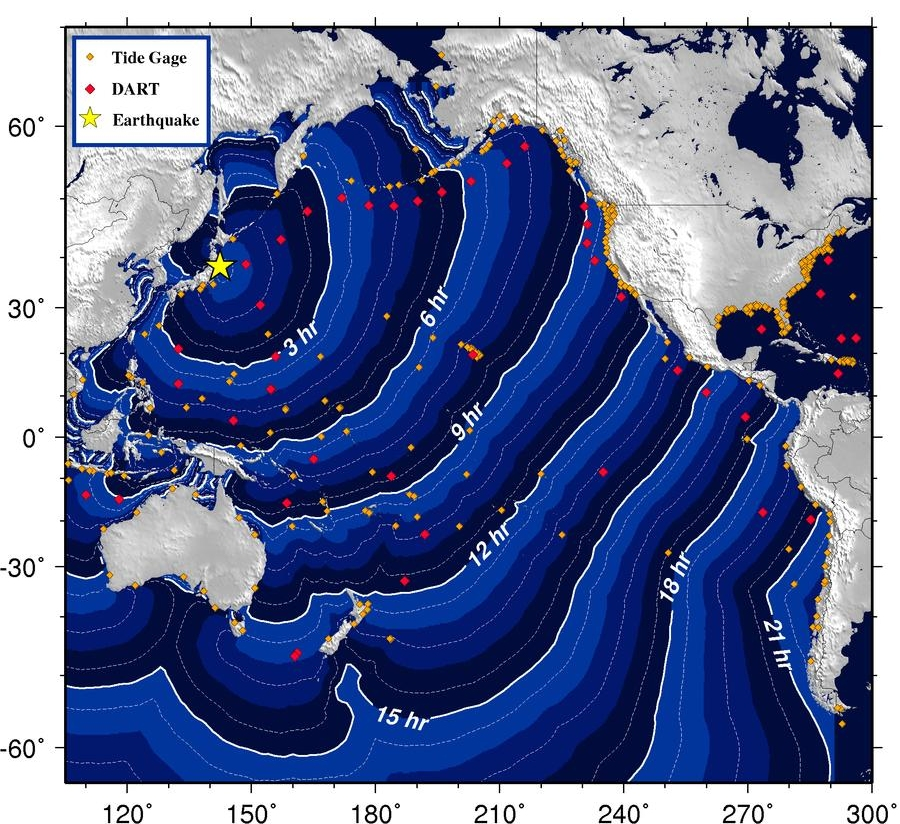
\includegraphics[width=\hsize]{../common/graphics/sendainoaa}
\end{center}
\caption{
Propagation of the tsunami caused by the Sendai earthquake on march 11 2011
based on a simulation by NOAA.
Hawai and other islands reduce the depth and thus the speed of propagation
of the wave.
Also apparent the shadowing of the wave due to obstacles like New Zealand.
\label{tsunamiausbreitung}}
\end{figure}

\begin{figure}
\begin{center}
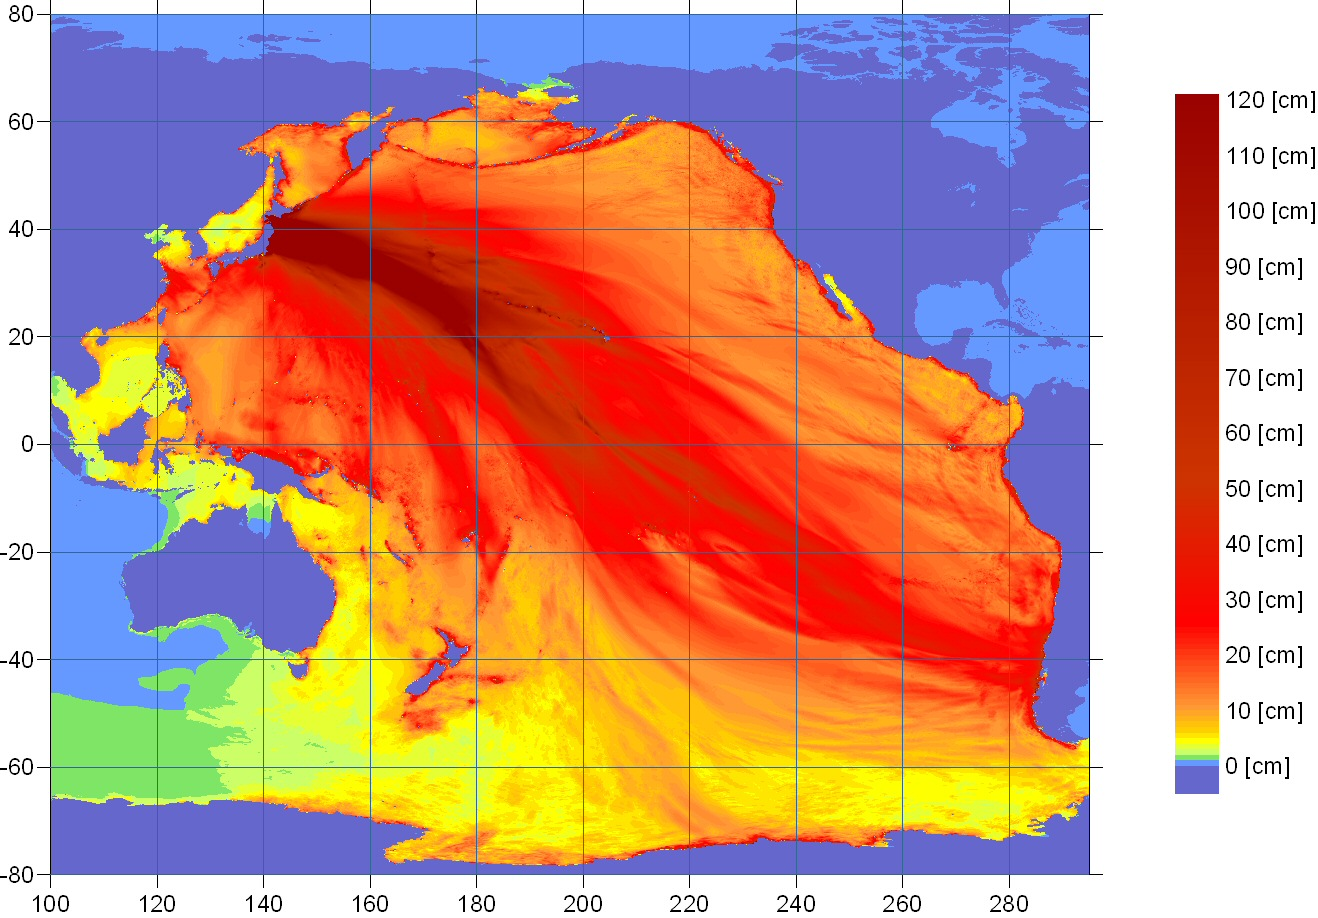
\includegraphics[width=\hsize]{../common/graphics/sendaienergy}
\end{center}
\caption{
Amplitude of the tsuname of march 11 2011.
Note that the great circles along which the waves propagate are mapped
to S-shaped durves.
Close to the coast the amplitude increases because of the reduced depth
and thus reduced velocity.
\label{tsunamienergie}}
\end{figure}

\subsection{Coordinates and boundary conditions}
We are interested in a wave originating in a single point, the
epicenter of the earthquake.
The solution in the idealized situation will necessarily be rotationally
symmetric around the axis through the epicenter.

We use spherical coordinates $(r,\vartheta,\varphi)$.
$\vartheta$ is the latitude measured from the north pole which will
also be the epicenter.
$\varphi$ is the longitude, a rotationally symmetric wave will not
depend on $\varphi$.
We can also neglect the $r$, as we consider only what happens at the
surface.
We therefore set $r=1$.

We are looking for a function
$u(t,\vartheta)$ satisfying initial conditions
\begin{align*}
u(0,\vartheta)&=F(\vartheta)\\
\frac{\partial}{\partial t}u(0,\vartheta)&=G(\vartheta).
\end{align*}

\subsection{Wave equation on the surface of a sphere}
The wave equation on the surface of a sphere can be obtained
by restricting the three dimensional wave equation
\[
\frac1{c^2} \frac{\partial^2}{\partial t^2}u =\Delta u.
\]
to the surface of the sphere.
We assume that units are chosen so that $c=1$, which amounts
to setting the time unit to time it takes for the wave to travel
one earth radius.

We can assume that the units are chosen in such a way that 
the $c=1$.
This can be accomplished by taking the radius of the earth as the
unit of length and the time it takes for the wave to travel one
earth radius as the unit of time.

The Laplacian must be expressedin spherical coordinates,
\[
\Delta u
=
\frac1{r^2} \frac{\partial}{\partial r}r^2\frac{\partial}{\partial r}u
+
\frac1{r^2\sin\vartheta}
\frac{\partial}{\partial\vartheta}
\sin\vartheta
\frac{\partial}{\partial\vartheta}
u
+
\frac1{r^2\sin^2\vartheta}\frac{\partial^2}{\partial\varphi^2}u
=
\frac1{\sin\vartheta}
\frac{\partial}{\partial\vartheta}
\sin\vartheta
\frac{\partial}{\partial\vartheta}
u
\]
The wave equation now turns into
\begin{equation}
\frac{\partial^2u}{\partial t^2}=
\frac1{\sin\vartheta}
\frac{\partial}{\partial\vartheta}
\sin\vartheta
\frac{\partial}{\partial\vartheta}
u=0.
\label{tsunami-gleichung}
\end{equation}

\subsection{Separation}
For the solution of the wave equation \eqref{tsunami-gleichung}
we now use the separation ansatz:
\[
u(t,\vartheta)=T(t)\Theta(\vartheta),
\]
and substitute it into the differential equation:
\[
T''(t)\Theta(\vartheta)=
T(t)
\frac1{\sin\vartheta}
\frac{d}{d\vartheta}
\sin\vartheta
\frac{d}{d\vartheta}\Theta(\vartheta)
\]
Since we are looking for a solution that does not vanish identically,
we may assume that $T(t)$ and $\Theta(\vartheta)$ only vanish in isolated
points so that we can divide by $T(t)\Theta(\vartheta)$ almost everywhere.
This allows us to separate the variables we were looking for:
\begin{equation}
\frac{T''(t)}{T(t)}
=
\frac1{\Theta(\vartheta)}
\frac1{\sin\vartheta}
\frac{d}{d\vartheta}
\sin\vartheta
\frac{d}{d\vartheta}\Theta(\vartheta).
\label{tsunami-separiert}
\end{equation}
The left hand side depends only on $t$, the right hand side only on
$\vartheta$.
This implies that the both sides are constant, giving us two coupled equations
\begin{align}
T''(t)&=mT(t)
\label{tsunami:zeitabh}
\\
\frac1{\sin\vartheta}
\frac{d}{d\vartheta}
\sin\vartheta
\frac{d}{d\vartheta}\Theta(\vartheta)
&=m\Theta(\vartheta).
\label{tsunami:winkelabh}
\end{align}
We now have to figure out which values $m$ for which both equations
can have solutions with reasonable boundary conditions which we
then can use to superimpose arbitrary solutions.

\subsection{Time dependence}
The time dependence equation \eqref{tsunami:zeitabh} is an ordinary
oscillation equation.
The solutions must have oscillatory character, which is only possible
for $m<0$.
The general solution then becomes
\[
T_m(t)=a_m\cos\sqrt{-m}t+b_m\sin\sqrt{-m}t
\]

\subsection{Angular dependency}
The differential equation \eqref{tsunami:winkelabh} for $\Theta$
is a little bit unwieldy.
By replacing $\Theta(\vartheta)$ by a function $y(x)$
using the substitution $x=\cos\vartheta$.
The derivative with respect to $\vartheta$ can be converted into
a derivative with respect to $x$ using the chain rule:
\[
\frac{d}{d\vartheta}\Theta(\vartheta)
=\frac{dy(x)}{dx}\frac{dx}{d\vartheta}
=-\sin\vartheta \frac{d}{dx} y(x)
\]
Using this in the differential equation, we obtain
\begin{align*}
\frac1{\sin\vartheta}
(-\sin{\vartheta})\frac{d}{dx}\sin\vartheta (-\sin\vartheta)
\frac{d}{dx}y(x)
&=
\frac{d}{dx}\sin^2\vartheta\frac{d}{dx}y(x)\\
&=
\frac{d}{dx}(1-\cos^2\vartheta)\frac{d}{dx}y(x)\\
&=
\frac{d}{dx}(1-x^2)\frac{d}{dx}y(x).
\end{align*}
The function we are looking for is therefore a solution of the
differential equation
\begin{equation}
\frac{d}{dx}(1-x^2)\frac{d}{dx}y(x)
=
my(x)
\label{tsunamieigenwertproblem}
\end{equation}
The function $y(x)$ must be defined in the entire interval $[-1,1]$.
This isn't automatic, as one can see already in the case $m=0$.
In that case, the differential equation can be integrating 
twice:
\begin{align*}
\frac{d}{dx}(1-x^2)\frac{d}{dx}y(x)&=0\\
(1-x^2)\frac{d}{dx}y(x)&=C\\
\frac{d}{dx}y(x)&=\frac{C}{1-x^2}\\
y(x)&=C\int\frac{dx}{1-x^2}\\
&=\frac{C}2\int\frac{dx}{1-x}+\frac{C}2\int\frac{dx}{1+x}\\
&=-\frac{C}2\log(1-x)+\frac{C}2\log(1+x) +D\\
&=\frac{C}2\log\frac{1+x}{1-x} + D
\end{align*}
At both interval ends, the function increases beyond bounds
unless $C=0$.

Polynomials would certainly be well defined on the whole interval,
so we attempt to solve the equation with a function of the form
\[
y(x)=a_0+a_1+a_2x^2+\dots a_nx^n.
\]
Substituting this in the differential equation and keeping only
terms of degree $n$, i.~e.~with $x^n$, we get  $ma_nx^n$
on the right side of \eqref{tsunamieigenwertproblem}.
On the left side we get
\[
-\frac{d}{dx}x^2\frac{d}{dx}a_nx^n
=
-\frac{d}{dx}x^2na_nx^{n-1}
=
-\frac{d}{dx}na_nx^{n+1}
=
-n(n+1)a_nx^n
\]
It follows that $m=-n(n+1)$, the equation \eqref{tsunamieigenwertproblem}
can only be solved with a polynomial of degree $n$ for precisely those
values ov $m$.
The differential equation now becomes
\begin{equation}
\frac{d}{dx}(1-x^2)\frac{d}{dx}y(x)+n(n+1)y(x)=0
\label{legendredgl}
\end{equation}

\subsection{Legendre polynomials}
The differential equation \eqref{legendredgl} is known as the differential
equation for the legendre polynomials.
The legendre polynomail $P_n(x)$ is a polynomial solution of
\eqref{legendredgl} with boundary condition $P_n(1)=1$.
However, this condition does not yet uniquely determine the function.
The additional condition is imposed that the polynomials also be
orthogonal in the sense that
\[
\int_{-1}^1 P_k(x)P_l(x)\,dx=0\quad\text{für $k\ne l$}.
\]
This allows to construct a theory similar to fourier theory for
approximation of functions in the interval $[-1,1]$.
This then determines the polynomials uniquely.

The first six Legendre polynomials are
\begin{align*}
P_0(x)&=1\\
P_1(x)&=x\\
P_2(x)&=\frac12(3x^2-1)\\
P_3(x)&=\frac12(5x^3-3x)\\
P_4(x)&=\frac18(35x^4-30x^2+3)\\
P_5(x)&=\frac18(63x^5-70x^3+15x)
\end{align*}
Furthermore we have
\[
\int_{-1}^1 P_k(x)^2\,dx = \frac{2}{2k+1}.
\]

The basic monomials $x^n$ can recovered by linear combinations of Legendre
polynomials, thus every function on $[-1,1]$ that can be approximated by
polynomials can also be approximated by Legendre polynomials $P_n(x)$.

Similarly to Fourier theory, the coefficients can be found using an
integral.
For
\[
f(x)=\sum_{k\ge 0} c_k P_k(x)
\]
the integrals
\[
\int_{-1}^1 f(x)P_l(x)\,dx
=
\sum_{k\ge 0} c_k \int_{-1}^1 P_k(x)P_l(x)\,dx
=
\frac{2c_k}{2k+1}
\]
imply that
\[
c_k=\frac{2k+1}{2}\int_{-1}^1P_k(x)f(x)\,dx.
\]
The coefficients $c_k$ are ``Legendre-coefficients'', they represent
the function $f(x)$ as a Legendre polynomial just as Fourier coefficients
represent periodic functions.

\subsection{Initial conditions}
\index{Initial conditions}
Using the Legendre polynomials, we can now solve the wave equation for
arbitrary initial contitions.
The solution must have the form
\[
u(t, x)=\sum_{k=0}^{\infty}(a_k\cos \lambda_k t+b_k\sin\lambda_k t)P_k(x),
\]
with $\lambda_k=\sqrt{k(k+1)}$.
The coefficients must be determined from initial conditions, i.~e.~from
the functions $F(\vartheta)=f(x)$ and $G(\vartheta)=g(x)$.
The initial condition for $u(t,x)$ gives
\begin{align*}
u(0,x)
&=\sum_{k=0}^{\infty} a_kP_k(x)=f(x)
\end{align*}
For the partial derivative $\partial_tu(t,x)$ we similarly get
\begin{align*}
\frac{\partial}{\partial t}u(0,x)
&=\sum_{k=0}^{\infty} \lambda_k b_kP_k(x)=g(x)
\end{align*}
The coefficients $a_k$ and $b_k$ can be computed by
\begin{align*}
a_k&=
\frac{2k+1}{2}\int_{-1}^1 P_k(x)f(x)\,dx
\\
b_k&=
\frac{2k+1}{2\lambda_k}\int_{-1}^1P_k(x)f(x)\,dx.
\end{align*}

\subsection{Point source}
\begin{figure}
\begin{center}
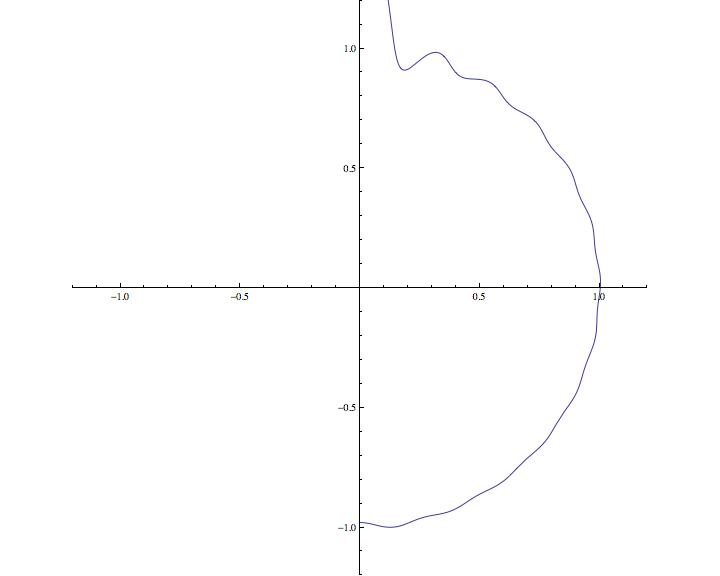
\includegraphics[width=\hsize]{../common/graphics/tsunami0}
\end{center}
\caption{Approximate solution for $N=25$ and $t=0$\label{tsunami0}}
\end{figure}
\begin{figure}
\begin{center}
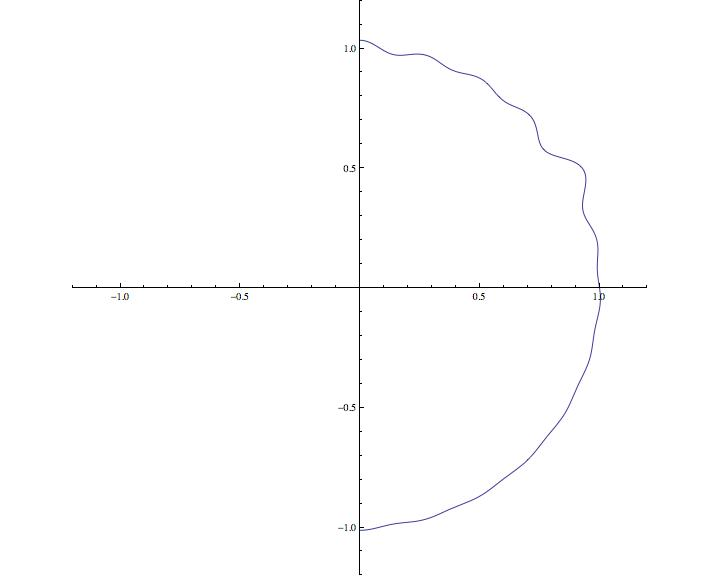
\includegraphics[width=\hsize]{../common/graphics/tsunami50}
\end{center}
\caption{Approximate solution for $N=25$ and $t=1$\label{tsunami50}}
\end{figure}
We now choose initial conditions that are supposed to approximate
what happens for an earthquake.
In a small neighborhood, the function is very large, but zero everywhere
else, but there is no initial velocity.
Thus we postulate that
\begin{align*}
f_\varepsilon(x)&=\begin{cases}
\frac1{\varepsilon}&\qquad 1-\varepsilon<x\le 1\\
0&\qquad\text{sonst}
\end{cases}
\\
g(x)&=0
\end{align*}
This allows to compute the coefficients.
The $b_k$ vanish, only the $a_k$ remain to be computed:
\begin{align*}
a_k(\varepsilon)&=\frac{2k+1}{2}\int_{-1}^1P_k(x)f_\varepsilon(x)\,dx
\\
&=\frac{2k+1}{2}\int_{1-\varepsilon}^1P_k(x)\frac1{\varepsilon}\,dx
\end{align*}
We are mainly interested in the situation where $\varepsilon$ is
very small, so we take the limit $\varepsilon\to 0$
\begin{align*}
\lim_{\varepsilon\to 0} a_k(\varepsilon)
&=
\frac{2k+1}{2}\lim_{\varepsilon\to 0}\frac1{\varepsilon}\int_{1-\varepsilon}^1P_k(x)\,dx
\end{align*}
Using the antiderivative $I_k(x)$ of $P_k(x)$ this becomes
\begin{align*}
\lim_{\varepsilon\to 0} a_k(\varepsilon)
&=
\frac{2k+1}{2}\lim_{\varepsilon\to 0}\frac{I_k(1)-I_k(1-\varepsilon)}{\varepsilon}
\\
&=\frac{2k+1}{2}I_k'(1)=\frac{2k+1}{2}P_k(1)=\frac{2k+1}{2}
\end{align*}
Formally, the solution thus is
\begin{equation}
u(t,x)
=
\sum_{k=0}^\infty \frac{2k+1}{2}P_k(x) \cos \sqrt{k(k+1)}t.
\end{equation}
Unfortunately, this series does not converge, which is not too
surprising given the very special initial conditions.
If we take only $N$ terms and renomarmlize with the factor $\frac1{N^2}$,
we get an approximate idea for the wave propagation.
Figures \ref{tsunami0} and \ref{tsunami50} show the series terminated 
after $25$ terms.

%
% jacobi.tex -- Anwendung: Hamilton-Jacobi-Formulierung der Mechanik
%
% (c) 2012 Prof Dr Andreas Mueller, Hochschule Rapperswil
% $Id$
%
\section{Anwendung: Hamiltonsche Mechanik\label{hamilton-mechanik}}
In den bisherigen Bespielen wurde jeweils ein Separationsansatz mit
einem Produkt von Teilfunktion gew"ahlt.
Dieser Abschnitt soll illustrieren, dass in einigen F"allen auch
ein Separationsansatz mit einer Summe von Teilfunktionen
zum Ziel f"uhren kann.
Dieser Fall ist f"ur die Anwendungen recht wichtig, denn die
dabei entstehende partielle Differentialgleichungen hat eine
gen"ugend einfach Struktur, dass der erste Separationsschritt immer
durchgef"uhrt werden kann.

\subsection{Motivation}
\index{Newtonsche Gesetze}
\index{Planeten}
\index{Satelliten}
Die Newtonschen Gesetze reichen vollst"andig, um die Bewegung von
Planeten und Satelliten vorherzusagen.
Unterliegt
ein K"orper der Masse $m$ mit zeitabh"angigen Koordinaten $\vec x(t)$
einer ortsabh"angigen Kraft $\vec F(\vec x)$, dann muss die Bahnkurve 
$\vec x(t)$ die gew"ohnliche Differentialgleichung
\begin{equation}
m\frac{d^2}{dt^2}\vec x(t)=\vec F(\vec x(t))
\label{jacobi:newton}
\end{equation}
erf"ullen. Ausgehend von einem bekanten Anfangspunkt $\vec x_0$ und
der Anfangsgeschwindigkeit $\vec v_0$ l"asst sich durch
l"osen der Differentialgleichung die Bahnkurve bestimmen.

Diese Beschreibung hat jedoch ein paar praktisch bedeutsame Nachteile.
Oft ist das Kraftgesetz nicht exakt bekannt. Zum Beispiel werden
Satelliten in niedrigem Erdorbit\footnote{Low earth orbit, wenige 100km}
\index{Erdorbit}
von der zwar sehr d"unnen, aber nicht vernachl"assigbaren
Erdatmosph"are abgebremst.
\index{Erdatmosphare@Erdatmosph\"are}
\index{Merkur}
Oder der Planet Merkur ver"andert laufend seine Bahn um einen winzigen
Betrag, ein Effekt, den erst Albert Einstein mit seiner speziellen
Relativit"atstheorie erkl"aren konnte.
Man sieht sich also oft mit der Aufgabe konfrontiert, dass man zwar die
Bahn berechnen k"onnte, wenn das Kraftgesetz exakt zutreffen w"urde,
dass man aber die Bahnver"anderungen unter dem Einfluss kleiner
Abweichungen vom exakten Kraftgesetz bestimmen sollte.
\index{Luftwiderstand}

\begin{beispiel}
\index{Billardtisch}
Als Beispiel betrachten wir ein Kugel auf einem ideal horizontal angenommenen
Billardtisch. Die Bewegung dieser Kugel wird offenbar genau beschrieben
durch den Anfangspunkt und die Geschwindigkeit $\vec x_0$ und $\vec v_0$.
Die Kugel wird in Richtung $\vec x_0$ weiterrollen, dabei
aber langsamer werden und schliesslich zum Stillstand kommen.
Es gibt also eine Kurve $t\mapsto \vec x(t, \vec x_0, \vec v_0))$,
die beiden Vektoren $\vec x_0$ und $\vec v_0$ bestimmen die
Bahn vollst"andig.

Was passiert, wenn der Billiardtisch nicht exakt horizontal ist?
Offenbar wirkt dann eine kleine zus"atzlich Kraft auf die Billard-Kugel,
und zwar in Richtung der gr"ossten Neigung der Billardtischplatte.
Wenn die Neigung sehr klein ist, ist die Abweichung von 
$\vec x(t,\vec x_0,\vec v_0))$ sehr gering.
Man k"onnte die Beschreibung diese Modifikation dadurch beschreiben,
dass man $\vec x_0$ und $\vec v_0$ leicht anpasst.
Die tats"achliche Position der Kugel zur Zeit $t$ ist die Position,
die eine Billiardkugel auf einem horizontalen Tisch ausgehend von
einem etwas anderen Ausgangspunkt $\vec x_0(t)$ mit einer
etwas anderen Ausgangsgeschwindigkeit $\vec v_0(t)$
nach Zeit $t$ erreicht h"atte.
\end{beispiel}

Der Vorteil dieser Beschreibung besteht darin, dass sich die
Abweichung vom exakten Kraftgesetz direkt in der Zeitabh"angigkeit
von $x_0(t)$ und $v_0(t)$ ausdr"uckt. Ist das Kraftgesetz exakt
erf"ullt, bleiben $x_0(t)$ und $v_0(t)$ konstant. Ausserdem ist die
Berechnung der Bahn ganz einfach: zu $\vec x_0$ kommt einfach
ein Vielfaches von $\vec v_0$ hinzu.

Die Bahnen der Satelliten sind offenbar viel komplizierter. 
Ort und Geschwindigkeit sind nicht geeignet, die
Bahn auf diese Art und Weise zu charakterisieren, sie "andern laufend
dramatisch ihre Gr"osse. Niemand kann mit Leichtigkeit sagen, ob
die Bahn vom Punkt  $\vec x_0$ mit Anfangsgeschwindigkeit $\vec v_0$
irgendwie "ahnlich aussieht wie die Bahn vom Punkt $\vec x_1$
mit Anfangsgeschwindigkeit $\vec v_1$.

\begin{aufgabe}
\label{jacobi:aufgabe}
Zu einem beliebigen mechanischen System finde man einen Satz von 
Parametern 
$Q_i$ und $P_i$ so, dass sich {\em jede}
Bahn mit Hilfe dieser Parameter in der Form
\begin{equation}
x_i(t) = x_i(t,Q_1,\dots,Q_n,P_1,\dots,P_n)
\label{jacobi:aufgabekurve}
\end{equation}
beschreiben l"asst.
\end{aufgabe}

\begin{beispiel}
Betrachten wir wieder das Problem der Billardkugel, aber nehmen wir
diesmal an, dass die Kugel ohne Reibung rollt. Dann gilt
\begin{equation}
\begin{aligned}
x(t)&=x_0 + tv_{x0},\\
y(t)&=y_0 + tv_{y0}.
\end{aligned}
\label{jacobi:linear}
\end{equation}
In dieser Form ist das bereits eine L"osung der gestellten Aufgabe,
denn jede Bahnkurve l"asst such durch geeignete Wahl der
Parameter $\vec x_0$ und $\vec v_0$ charakterisieren.

Man kann aber noch mehr erreichen: man kann die Koordinaten $Q_i$ und $P_i$
so w"ahlen, dass die $P_i$ alle die Bedeutung einer Energie,
und die $Q_i$ die Bedeutung einer Zeit haben.
Die Funktion der $P_i$ k"onnen die Terme
\begin{equation*}
\begin{aligned}
P_x&=\frac12mv_x^2,&
P_y&=\frac12mv_y^2
\end{aligned}
\end{equation*}
"ubernehmen, also die Beitr"age der Bewegungskomponenten in $x$-
bzw.~$y$-Richtung zur Energie. Da die Kugel reibungsfrei rollt, sind
diese Gr"ossen konstant.

Die Gr"ossen $Q_x$ und $Q_y$ m"ussen so gew"ahlt werden, dass 
die Gleichungen (\ref{jacobi:linear}) die tats"achliche Bahn beschreiben.
Durch Aufl"osen von (\ref{jacobi:aufgabekurve}) nach $Q_i$ findet man
\begin{equation*}
\begin{aligned}
Q_x&=-\frac{x_0}{v_{0x}},\\
Q_y&=-\frac{y_0}{v_{0y}}.
\end{aligned}
\end{equation*}
Die Zahlen $-Q_x$ und $-Q_y$ sind also die Zeiten, zu denen die
Billardkugel die $x$- bzw.~$y$-Achse kreuzt.
\end{beispiel}

Die schwierigere Frage ist, ob jedes mechanische System eine
L"osung der Aufgabe \ref{jacobi:aufgabe} zul"asst.
Die Antwort passt ins Thema: ja, man kann eine solche Beschreibung
finden, aber man muss dazu die L"osung einer speziellen
partiellen Differentialgleichung finden. Oft l"asst sich die
Differentialgleichung mit einem Separationsansatz l"osen.

\subsection{Hamilton-Jacobi-Formalismus}
\index{Hamilton-Jacobi-Formalismus}
In der Hamiltonschen Beschreibung der Mechanik geht man aus von
der Gesamtenergie $H(x_i, p_i)$ ausgedr"uckt durch Ort und Impuls.
F"ur das Beispielproblem ist
\index{Hamilton-Funktion}
\begin{equation}
H(x_i,p_i)=\frac1{2m}(p_x^2+p_y^2).
\label{jacobi:hamilton:funktion}
\end{equation}
Der Zusammenhang zwischen den Koordinaten und den Impulsen ist dann
durch die Hamiltonschen Differentialgleichungen gegeben:
\begin{align}
\frac{d}{dt}x_i&=\frac{\partial H}{\partial p_i}
&\Rightarrow
\qquad \dot x_i&=\frac{p_i}{m}=v_i
\label{jacobi:hamilton:geschwindigkeit}
\\
\frac{d}{dt}p_i&=-\frac{\partial H}{\partial x_i}
&\Rightarrow
\qquad
\dot p_i&=m\ddot x_i=0
\label{jacobi:hamilton:newton}
\end{align}
\index{Hamilton-Gleichungen}
Die erste Gleichung (\ref{jacobi:hamilton:geschwindigkeit}) stellt
nur den Zusammenhang zwischen der Geschwindigkeit und dem Impuls
her. Die zweite Gleichung (\ref{jacobi:hamilton:newton}) besagt in
diesem Fall, dass keine Kraft wirkt. N"ahme man in 
(\ref{jacobi:hamilton:funktion}) noch ein Potential $V(x)$ hinzu,
w"urde die zweite Gleichung zu
\[
m\ddot x_i=-\frac{\partial V}{\partial x_i} = F_i(x),
\]
also genau dem Newtonschen Gesetz.

Nach Hamiliton ist jeder andere Satz von Koordinaten $Q_i$ und $P_i$
genauso geeignet zur Beschreibung des mechanischen Systems, solange die
Gleichungen 
(\ref{jacobi:hamilton:geschwindigkeit}) und (\ref{jacobi:hamilton:newton})
weiterhin G"ultigkeit haben. Jacobi und Hamilton haben eine Methode
angegeben, mit der man eine Koordinatentransformation finden kann.

\begin{satz}
\label{jacobi:satz}
Eine L"osung der Aufgabe (\ref{jacobi:aufgabe}) wird gefunden mit
Hilfe einer Funktion $S(x_i, t)$, die L"osung der partiellen
Differentialgleichung
\begin{equation}
\frac{\partial S}{\partial t}
=
H\biggl(
x_i,
\frac{\partial S}{\partial x_i}
\biggr)
\label{jacobi:hamilton:dgl}
\end{equation}
erf"ullt.
Eine L"osungsfunktion $S$ der Differentialgleichung enth"alt notwendigerweise
ein Anzahl von Integrationskonstanten $P_i$.
Die partiellen Ableitungen von $S$ nach diesen $P_i$
sind die neuen konstanten Bahnparameter $Q_i$
\begin{equation}
Q_i=\frac{\partial S}{\partial P_i}
\label{jacobi:hamilton:impuls}
\end{equation}
Die Gleichungen (\ref{jacobi:hamilton:impuls}) enthalten ausser den
Gr"ossen $P_i$ und $Q_i$ auch die Koordinaten $x_i$ und die Zeit $t$.
Durch Aufl"osen nach den Variablen $x_i$ l"asst sich die Bahnkurve
als Funktion
\[
x_i(t,Q_i,P_i)
\]
ausdr"ucken.
\end{satz}
Der Parametersatz $(Q_i,P_i)$ beschreibt also alle m"oglichen 
Bahnen. Zwei Bahnen k"onnen sehr einfach verglichen werden, wenn die
Paramter $Q_i$ und $P_i$ nahe beeinander sind, dann liegen auch
die Bahnen nahe beeinander.

Eine Begr"undung f"ur diesen Satz liegt ausserhalb der Ziele
dieser Vorlesung, wir wollen aber mit zwei Beispielen zeigen,
dass dieser Formulismus funktioniert und die L"osung der
Bewegungsdifferentialgleichungen des Systems erm"oglicht.

\subsection{Energieerhaltung}
Ein Spezialfall ist von besonderer Bedeutung. In einem abgeschlossenen
System ist die Energie erhalten, die Hamilton-Funktion $H$, die ja
die Energie darstellt, kann also nicht von der Zeit abh"angen.
Verwenden wir einen Separationsansatz der Form 
\[
S(t,x_i)=S_0(t)+S_1(x_1)+\dots+S_n(x_n),
\]
wird die Hamilton-Jacobi-Differentialgleichung zu
\[
S_0'(t)=H(S_1'(x_1),\dots, S_n'(x_n)).
\]
Die linke Seite h"angt nur von $t$ ab, auf der rechten Seite
kommt $t$ aber gar nicht vor, die Variablen $t$ und $x_i$ sind
separiert, beide Seiten der Gleichung m"ussen konstant sein.
Wir nennen die Konstante $P_1$, sie ist der Wert der Hamilton-Funktion,
also die Gesamtenergie.
Damit steht auch schon fest, dass die gesuchte Funktion $S(t, x_i)$
die Form
\[
S(t,x_i)=P_1t + \bar S(x_i)
\]
haben muss, wobei $\bar S(x_i)$ die Zeit $t$ nicht enthalten kann.
F"ur die Koordinaten $Q_i$ gilt daher
\begin{align*}
Q_1&=\frac{\partial S}{\partial P_1}=t+\frac{\partial \bar S(x_i)}{\partial P_1},
\\
Q_i&=\frac{\partial \bar S}{\partial P_i},\qquad i>1
\end{align*}
Die Gleichungen f"ur $Q_i$ mit $i>1$ enthalten die Zeit nicht, sie
beschreiben also ausschliesslich die Form der Bahn in Abh"angigkeit
von den Parameter $Q_1,\dots,Q_n,P_1,\dots,P_n$. Die erste
Gleichung ist die einzige, die Zeit enth"alt. In ihrem zweiten
Term kommt die Zeit ebenfalls nicht vor, sondern nur die Ortskoordinaten.
Die Ortskoordinaten h"angen daher nur von
\[
t-Q_1,Q_2,\dots,Q_n, P_1,\dots,P_n
\]
ab. Statt der Form (\ref{jacobi:aufgabekurve}) gibt es also sogar eine
L"osung der Form
\[
x_i(t)=x_i(t-Q_1,Q_2, \dots,Q_n,P_1,\dots,P_n).
\]

F"ur eine Punktmasse in drei Dimensionen k"onnen wir also schliessen, 
dass es immer eine Beschreibung der Bahn mit sechs Parametern
$Q_1,Q_2,Q_3,P_1,P_2,P_3$ gibt, wobei der Parameter $Q_1$ die Bedeutung
hat, dass ein ganz bestimmter, geometrisch ausgezeichneter Bahnpunkt
zu dieser Zeit durchlaufen wird.
Bei der Beschreibung von Planetenbahnen dieser Punkt typischerweise
das Perihel, der Sonnenn"achste Punkt, oder bei Satelliten entsprechend
das Perig"aum, der erdn"achste Punkt.

\subsection{Beispiele}
\subsubsection{Bewegung ohne "ausseren Krafeinfluss in zwei Dimensionen}
\index{Bewegung ohne Krafteinfluss}
Wir beginnen wieder bei der Hamilton-Funktion 
\[
H(p_x, p_y)=\frac1{2m}(p_x^2+p_y^2).
\]
Nach (\ref{jacobi:hamilton:dgl}) m"ussen wir jetzt also die
Differentialgleichung
\[
\frac1{2m}\biggl(
\biggl(\frac{\partial S}{\partial x}\biggr)^2
+
\biggl(\frac{\partial S}{\partial y}\biggr)^2
\biggr)=\frac{\partial S}{\partial t}
\]
f"ur die Funktion $S(t,x,y)$ l"osen. Wir verwenden dazu einen 
Separationsansatz der Form
\[
S(t,x,y)=S_1(x)+S_2(y) + S_3(t).
\]
Einsetzen in die Differentialgleichung liefert
\begin{equation}
\frac1{2m}( S_1'(x)^2+S_2'(y)^2)=S_3'(t).
\label{jacobi:kraeftefrei:sep1}
\end{equation}
Die linke Seite h"angt nicht von $t$ ab, die rechte h"angt
aber nur von $t$ ab, also sind beide Seiten konstant.
Wir nennen die Konstanten $P_1$. Damit l"asst sich
jetzt $S_3(t)$ bestimmen, es muss eine geeignete Integrationskonstante
geben, so dass
\[
S_3(t)=P_1t
\]
damit ist die Aufgabe \ref{jacobi:aufgabe} mindestens f"ur die Variable
$t$ bereits gel"ost.

Wir untersuchen jetzt die linke Seite von (\ref{jacobi:kraeftefrei:sep1}).
Auch diese Gleichung kann man unter Verwendung der Konstanten $P_1$
separieren:
\[
\frac1{2m} S_1'(x)^2
=
P_1-\frac1{2m}S_2'(y)^2.
\]
Die linke Seite h"angt nur von $x$ ab, die rechte nur von $y$, also
sind beide konstant. 
Wir nennen die Konstante $P_2$ und finden die L"osung
\[
S_1(x)
=
\sqrt{2mP_2}x.
\]
Jetzt kann man aber auch noch $S_2$ bestimmen. Es ist n"amlich 
\[
\frac1{2m} S_2'(y)^2
=P_1-P_2
\]
woraus sich wie vorhin die L"osung
\[
S_2(y)
=
\sqrt{2m(P_1-P_2)}y
\]
ergibt. Damit haben wir jetzt eine L"osung der Differentialgleichung:
\[
S(x,y,t)=
P_1t
+
\sqrt{2mP_2}x
+
\sqrt{2m(P_1-P_2)}y
\]
Nach den Regeln des Satzes \ref{jacobi:satz}, sind die zu verwendenden
Koordinaten die partiellen Ableitungen:
\begin{align*}
Q_1&=\frac{\partial S}{\partial P_1}
=
t + \sqrt{\frac{m}{2(P_1-P_2)}}y,\\
Q_2&=\frac{\partial S}{\partial P_2}
=
\sqrt{\frac{m}{2P_2}}x
-
\sqrt{\frac{m}{2(P_1-P_2)}}y
\end{align*}
Jetzt kann man nach $x$ und $y$ aufl"osen und damit die
Bahnkurve durch die Konstanten $Q_i$ und $P_i$ und die Zeit $t$
ausdr"ucken:
\begin{align*}
x&=\sqrt{\frac{2P_2}{m}}(Q_1+Q_2-t)\\
y&=\sqrt{\frac{2(P_1-P_2)}{m}}(Q_1-t).
\end{align*}
Wie erwartet beschreiben diese Gleichungen eine gleichf"ormige
Bewegung. Die Geschwindigkeit ist die Ableitung nach der Zeit,
also
\begin{align*}
v_x
&=
\sqrt{\frac{2P_2}{m}}
&\Rightarrow&&
P_2&=\frac{mv_x^2}2
\\
v_y
&=
\sqrt{\frac{2(P_1-P_2)}{m}}
&\Rightarrow&&
P_1&=P_2+\frac{mv_y^2}2=\frac{m}2(v_x^2+v_y^2)=\frac12mv^2
\end{align*}
Die physikalische Bedeutung von $P_1$ ist also die kinetische
Energie des
Gesamtsystems, w"ahrend $P_2$ die kinetische Energie darstellt, die in
der Bewegungskomponent in $x$-Richtung steckt.

\subsubsection{Schiefer Wurf}
\index{schiefer Wurf}
Wir betrachten den schiefen Wurf, der sich vom vorangegangenen
Beispiel durch ein zus"atzliches Gravitationspotential
unterscheidet. Die Gesamtenergie ist jetzt
\[
H(x,y,t)=\frac1{2m}(p_x^2+p_y^2)+mgy.
\]
Die Hamilton-Jacobi-Differentialgleichung lautet jetzt
\[
\frac1{2m}\biggl(
\biggl(\frac{\partial S}{\partial x}\biggr)^2
+
\biggl(\frac{\partial S}{\partial y}\biggr)^2
\biggr)
+mgy=\frac{\partial S}{\partial t} 
\]
Der selbe Separationsansatz wie vorhin f"uhrt auch wieder zu
\[
\frac1{2m}(S_1'(x)^2+S_2'(y)^2)+mgy=S_3'(t),
\]
woraus wieder folgt, dass $S_3'(t)=P_1$ konstant ist.

Wir k"onnen aber auch $x$ und $y$ separieren:
\begin{align*}
\frac1{2m}S_1'(x)^2&=P_1-\frac1{2m}S_2'(y)^2-mgy
%\\
%\frac1{\sqrt{2m}}S_1'(x)&=\sqrt{P_3-\frac1{2m}S_2'(y)^2+mgy}
\end{align*}
Die linke Seite h"angt nicht von $y$ ab, die rechte nicht von $x$, also sind
beide konstant, wir nennen die Konstante $P_2$, und bekommen
die L"osung $S_1=\sqrt{2mP_2} x$.

Die rechte Seite k"onnen wir jetzt auch l"osen:
\begin{align*}
P_2&=
P_1-\frac1{2m}S_2'(y)^2-mgy
\\
\frac1{2m}S_2'(y)^2
&=
P_1-P_2-mgy
\\
S_2'(y)&=\sqrt{
2m(P_1-P_2-mgy)
}
\\
S_2(y)
&=
\frac1{3m^2g}\bigl(2m(P_1-P_2-mgy)\bigr)^{\frac32}
\end{align*}
Damit ist jetzt eine L"osungsfunktion $S(x,y,t)$ vollst"andig
bekannt:
\[
S(x,y,t)=P_1t+\sqrt{2mP_2}x +
\frac1{3m^2g}\bigl(2m(P_1-P_2-mgy)\bigr)^{\frac32}
\]
Die zu verwendenden Koordinaten bekommt man jetzt wie vorhin durch
partielle Ableitung nach den $P_i$. Man bekommt nacheinander:
\begin{equation}
\begin{aligned}
Q_1=\frac{\partial S}{\partial P_1}
&=
t+
\frac1{g}\sqrt{\frac{2(P_1-P_2-mgy)}{m}}
\\
Q_2=\frac{\partial S}{\partial P_2}
&=
\sqrt{\frac{m}{2P_1}}x
-
\frac1{g}\sqrt{\frac{2(P_1-P_2-mgy)}{m}}
\end{aligned}
\label{jacobi:aufloesung}
\end{equation}
Die erste Gleichung kann man nach $y$ aufl"osen:
\begin{equation}
y=
\frac{P_1-P_2}{mg}-\frac{g}{2}(Q_1-t)^2
\label{jacobi:quadratisch}
\end{equation}
Die H"ohe h"angt quadratisch von der Zeit ab, $Q_1$ ist die Zeit
der gr"ossten H"ohe, die Scheitelzeit.

Die Aufl"osung nach $x$ wird einfacher, wenn man erst die Summe der beiden
Gleichungen (\ref{jacobi:aufloesung}) bildet:
\begin{align*}
Q_1+Q_2&=t+\sqrt{\frac{m}{2P_1}}x\\
x&=\sqrt{\frac{2P_1}{m}}(Q_1+Q_2-t)
\end{align*}
Die $x$-Koordinate nimmt offenbar linear mit der Zeit zu. Die
Geschwindigkeit ist
\[
v_x=\sqrt{\frac{2P_1}{m}}\quad\Rightarrow\quad P_1=\frac{mv_x^2}2,
\]
$P_1$ ist also die kinetische Energie der Horizontalbewegung.
$Q_2$ gibt an, wie viel Zeit nach dem Scheiteldurchgang die $x$-Koordinate
verschwindet.

Zur Zeit $t=Q_1$ verschwindet der quadratische Term in
(\ref{jacobi:quadratisch}), und man kann die Gleichung vereinfachen
zu 
\[
mgy + P_2=P_1.
\]
Da $P_2$ die kinetische Energie der Horizontalbewegung ist, und $mgy$
die potentielle Energie, ist $P_1$ wie erwartet die Gesamtenergie.


